%!TEX root = ../prueba.tex

En este capítulo se describen y definen a los actores que van a utilizar el sistema, los cuales se pueden observar en la figura \ref{fig:actores}. La descripción de estos actores es tomando como base el organigrama generalizado de una cafetería que se plantea en el documento \textit{E01-Especificación del Proyecto} el cual se puede observar en la figura \ref{fig:organigramaCafeteria}.

\begin{figure}[hbtp!]
	\begin{center}
		\fbox{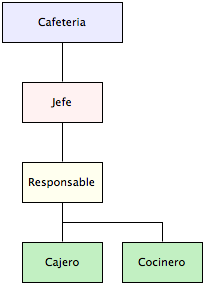
\includegraphics[width=0.3\textwidth]{img/organigrama}}
		\caption{Organigrama de una Cafetería}
		\label{fig:organigramaCafeteria}.
	\end{center}
\end{figure}

Así mismo se observa en la figura \ref{fig:actores} la presencia de un actor al que se le conoce como \getElementById[Stakeholder]{Agente} el cual hace referencia a un puesto de nuestra empresa \textbf{Loli Inc.} el cual pertenece al departamento de atención a usuarios, esto tomando como base el organigrama que se muestra en la figura \ref{fig:organigramaLoliInc}.

\begin{figure}[hbtp!]
	\begin{center}
		\fbox{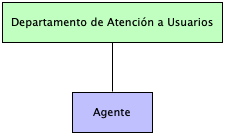
\includegraphics[width=0.3\textwidth]{img/organigramaLoliInc}}
		\caption{Organigrama de la empresa Loli Inc}
		\label{fig:organigramaLoliInc}
	\end{center}
\end{figure}


A continuación se realizan algunas observaciones correspondientes al diagrama en la figura \ref{fig:actores}:
	\begin{enumerate}
		\item El \getElementById[Stakeholder]{Persona} es un actor abstracto, que tiene como principal propósito abstraer las funcionalidades a las que todos las personas que utilicen el sistema tienen acceso sin depender directamente el rol que desempeñan. Por ejemplo, tanto el \getElementById{Cocinero} como el \getElementById{Cliente} tienen la misma posibilidad de Iniciar Sesión en el sistema o recuperar su cuenta de usuario asociada.
		\item El \getElementById[Stakeholder]{ResponsableDeLocal} es designado únicamente por el \getElementById{Jefe} y debe ser un empleado que puede o no tener el rol de \getElementById{Cocinero} o \getElementById{Cajero} en la misma cafetería.
	\end{enumerate}
	
	\begin{figure}[hbtp!]
	\begin{center}
		\fbox{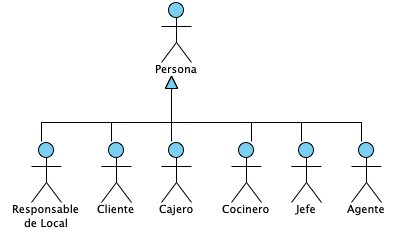
\includegraphics[width=0.5\textwidth]{img/actores}}
		\caption{Actores del Sistema}
		\label{fig:actores}
	\end{center}
\end{figure}


\begin{Actor}{Persona}{Persona}{Un usuario es toda persona que va a interactuar con el sistema mediante la aplicación móvil o la aplicación web.}
	\item[Responsabilidades:] No aplica.
	\item[Perfil]:\hspace{1pt}
		\begin{itemize}
			\item Alumno de nivel medio superior, superior o posgrado del I.P.N. o de U.N.A.M.
			\item Docente de nivel medio superior, superior o posgrado del I.P.N. o de U.N.A.M.
			\item Personal externo en una unidad académica del I.P.N. o escuela de la U.N.A.M.
			\item Personal de una cafetería.
		\end{itemize}
\end{Actor}


\begin{Actor}{Jefe}{Jefe}{También conocido como \textbf{Dueño} es la persona que legalmente tiene derecho a utilizar el nombre de una franquicia para abrir uno o más locales en determinados espacios, dentro o fuera de una unidad académica del I.P.N. así como una escuela de otra Institución Educativa.}
	\item[Responsabilidades:] \hspace{1pt}
		\begin{itemize}
			\item Agregar al sistema a los empleados.
			\item Designar un responsable del local.
			\item Tomar desiciones ejecutivas que respondan a las demandas de su establecimiento con base en 			gráficas o datos estadísticos.
			\item Definir las horas de operación de un local.
		\end{itemize}
	\item[Perfil]:\hspace{1pt}
		\begin{itemize}
			\item Licenciatura.
			\item Responsable.
			\item Líder.
		\end{itemize}
\end{Actor}

\begin{Actor}{ResponsableDeLocal}{Responsable de Local}{Es la persona designada por el \getElementById[Stakeholder]{Jefe} o Dueño para administrar o gestionar un local, recibir las entregas de productos de los proveedores con la facultad de delegar esta responsabilidad a otro empleado. }
	\item[Responsabilidades:] \hspace{1pt}
		\begin{itemize}
			\item Verificar que la integridad de los productos que llegan a la cafetería cumple con los acuerdos, reglamentos o estándares correspondientes.
			\item Definir las promociones que aplican a la cafetería de la que es responsable.
		\end{itemize}
	\item[Perfil]:\hspace{1pt}
		\begin{itemize}
			\item Licenciatura.
			\item Responsable.
			\item Confiable.
			\item Honesto.	
		\end{itemize}
\end{Actor}


\begin{Actor}{Cliente}{Cliente}{Es cualquier persona que va a una cafetería o local a consumir alimentos.}
	\item[Responsabilidades:]\hspace{1pt}
		\begin{itemize}
			\item Realizar el pago correspondiente a su pedido.
			\item Estar en el local al menos 5 minutos antes de que su pedido haya concluido su preparación.
			\item Revisar y responder a las notificaciones del sistema.
		\end{itemize}
	\item[Perfil:]\hspace{1pt}
		\begin{itemize}
		\item Alumno de nivel medio superior, superior o posgrado del I.P.N. o de U.N.A.M.
			\item Docente de nivel medio superior, superior o posgrado del I.P.N. o de U.N.A.M.
			\item Personal externo en una unidad académica del I.P.N. o escuela de la U.N.A.M.
		\end{itemize}
\end{Actor}


\begin{Actor}{Cocinero}{Cocinero}{Es una persona que pertenece a una cafetería y que tiene como principal responsabilidad atender pedidos y cocinarlos o delegarle esta responsabilidad a otro cocinero dentro de la misma cafetería.}
	\item[Responsabilidades:]\hspace{1pt}
		\begin{itemize}
			\item Monitoreo, control y conservación de los insumos de la cocina.
			
			\item Colaborar en la planificación de menús.
			
			\item Ayudar a administrar los costos e inventario.
			
			\item Dividir, conducir y organizar el trabajo con otros miembros del staff en la preparación de las ordenes.
			
			\item Iteractuar con el proveedor del servicio.
			
			\item Atender y preparar los pedidos solicitados por los clientes.
		\end{itemize}
	
	\item[Perfil:] \hspace{0.5cm}
		\begin{itemize}
			\item Excelentes habilidades de comunicación.
			
			\item Buenos estándares de higiene.
			
			\item Organizado y metódico.
			
			\item Experiencia en cáterin.
		\end{itemize}
\end{Actor}


\begin{Actor}{Cajero}{Cajero}{Es una persona que pertenece a una cafetería y que tiene como propósito cobrar los pedidos de los clientes.}
\item[Responsabilidades:] \hspace{0.5cm}
		\begin{itemize}
			\item Recibir dinero en efectivo, de requerirlo realiza arqueos de caja.
			
			\item Es el responsable directo de dinero en efectivo.
			
			\item Registrar operando una caja los movimientos de entrada y salida de dinero.
			
			\item Informar a su superior los movimientos diarios de la caja.
			
			\item Mantener en orden el equipo y sitio de trabajo, reportando cualquier anomalia.
			
			\item Manejar un grado de confidencialidad sobre las transacciones bajo.
		\end{itemize}
	
	\item[Perfil:] \hspace{0.5cm}
		\begin{itemize}
			\item Excelentes habilidades de comunicación , para atención al cliente.
			
			\item Habilidades numericas.
			
			\item Actitud de servicio.
			
			\item Proactivo.
			
			\item Responsable.
			
			\item Buena gestión de tiempo.
		\end{itemize}

\end{Actor}



\begin{Actor}{Administrador}{Administrador}{Es la persona que se encargará de desbloquear cuentas de usuario en el sistema así como de vigilar y mejorar las respuestas del sistema una vez sea puesto en producción.}
\item[Responsabilidades:]\hspace{1pt}
		\begin{itemize}
			\item Desbloquear cuentas de usuario.
		\end{itemize}
	\item[Perfil:]\hspace{1pt}
		\begin{itemize}
			\item Conocimiento en informática.
			\item Facilidad para comunicarse.
			\item Dominio y conocimiento básico de la funcionalidad del sistema.
		\end{itemize}

\end{Actor}


